

\ifdefined\maindoc
% Do nothing (we are inside main.tex)
\else
\documentclass[12pt]{report}
\usepackage[a4paper,margin=1in]{geometry}
\usepackage[utf8]{inputenc}
\usepackage[T1]{fontenc}
\usepackage{amsmath,amssymb,amsthm}
\usepackage{booktabs}
\usepackage{setspace}
\usepackage{graphicx}
\usepackage{subcaption}
\usepackage{enumitem}
\usepackage{placeins}
\usepackage{hyperref}
\usepackage{array}
\usepackage{makecell}
\usepackage{algorithm}
\usepackage{algpseudocode}
\usepackage[backend=biber,style=ieee,citestyle=numeric-comp,sorting=none]{biblatex}
\addbibresource{references.bib}
\newtheorem{theorem}{Theorem}
\newtheorem{lemma}[theorem]{Lemma}
\newtheorem{definition}[theorem]{Definition}
\newtheorem{proposition}[theorem]{Proposition}
\onehalfspacing
\graphicspath{{figures/}}
% Standalone-only fallbacks so Chapter~\ref{...} renders as the right number outside the
% main thesis. Under \maindoc these are skipped and the real labels in main.tex resolve.
\makeatletter
\newlabel{ch:input-module}{{3}{1}{}{Doc-Start}{}}
\newlabel{ch:diamond-module}{{4}{1}{}{Doc-Start}{}}
\newlabel{ch:probability-toolkit}{{5}{1}{}{Doc-Start}{}}
\makeatother
\begin{document}
\title{Information As Schedule and Cost: Critical Path Toolkit}
\fi

\newcommand{\comb}{\oplus}
\newcommand{\prop}{\otimes}

\section{Introduction}
\label{sec:cpm-intro}

The Critical Path Toolkit consumes the unified graph object of
Chapter~\ref{ch:input-module} directly and involves no decomposition. Every
analysis in it is built from linear-time passes over the layered iteration
sets, so the Network Decomposition Module of Chapter~\ref{ch:diamond-module}
is bypassed entirely.

The quantities this toolkit propagates are the ones that accumulate along
dependency paths. A duration, a cost, a risk factor and a load all compound
as they travel, and a network carrying such a quantity poses the same pair
of questions whatever the quantity is. One is extremal, asking for the best
or worst value a complete chain of dependencies can produce. The other
concerns room, asking how far an individual component can move before that
extremal answer changes. The first is settled by a forward pass. The second
is where the analysis actually lives, because room is what criticality,
bottlenecks and priorities are made of, and it exists only where the
arithmetic of the quantity can be run backwards.

\section{Scheduling Analysis on Networks}
\label{sec:cpm-grounding}

The critical path method models a project as a network of activities and
computes the longest path through it. The project cannot finish earlier than
that path allows, the activities on it have no room to slip, and every other
activity carries a float equal to how far it can slip before it starts to
matter. The method and the float calculus date to the late 1950s
\cite{kelley1959critical}, and the companion question of duration uncertainty
was raised almost immediately: PERT replaced each fixed duration with a
three-point estimate and a distributional assumption
\cite{malcolm1959pert}, and its descendants in modern practice replace the
assumption with Monte Carlo sampling. Distribution-free treatment of the same
uncertainty came much later. When each duration is known only as an interval,
the forward quantities remain easy, but the backward ones change character
entirely. Deciding whether an activity is possibly critical is NP-complete
and float bounds are NP-hard \cite{chanas2002complexity}, even on planar
networks \cite{chanas2003planar}. Exact methods exist for latest starting
times and one of the two float bounds \cite{dubois2005floats}, the
consolidated picture is given by Fortin, Zieli\'{n}ski, Dubois and Fargier
\cite{fortin2010criticality}, and the recognised tractable class is the
series--parallel networks.

None of the machinery is specific to time. The forward recursion combines
incoming values and compounds them along edges, and any quantity with those
two operations propagates the same way. With combination as maximum and
compounding as addition the recursion is the critical path method. With other
pairs it is cost roll-up, risk scaling or route selection, and the algebra of
such systems is well established: max-plus linear systems theory treats the
classical forward and backward passes as linear algebra over an idempotent
semiring, with the backward pass arising as residuation
\cite{baccelli1992sync}. The lesson of that algebra is a discipline. A
forward recursion exists for any pair of operations, but a backward one is a
property the pair either has or lacks, and an analysis that reports slack
without checking has manufactured a number. Uncertainty sharpens the same
discipline from another side, because the interval results above draw their
line between easy and hard exactly where monotonicity is lost.

\section{Analysis Modes}
\label{sec:cpm-modes}

Whether the room question has an answer is a property of the operator pair,
and it has one in exactly two situations. When combination is an order,
maximum or minimum, a bound on the combined value binds every argument, and
when compounding is monotone with a residual the bound inverts across each
edge, so a constraint of the form finish by $K$ travels backwards through
the network the same way values travel forwards. That is residuation in an
idempotent semiring \cite{baccelli1992sync}, and it is what the classical
backward pass has always been. Summation is different in kind. A total is
not a deadline and no residuation exists, but a summed system is linear,
and a linear map has an adjoint. The backward object of an accumulation
analysis is therefore a sensitivity, and the room it measures is an
allowance against a stated budget rather than a slack against a deadline.
A pair with neither structure supports a forward recursion and nothing
else, and any margin reported for it would be invention. A configuration of
the toolkit, called a mode, is an operator pair together with whatever
backward semantics its algebra supports, and Table~\ref{tab:cpm-modes}
lists the four the framework provides.

\begin{table}[htbp]
\centering
\caption{The shipped modes. Every row carries a defined backward semantics;
the margin column names what the backward pass reports.}
\label{tab:cpm-modes}
\small
\renewcommand{\arraystretch}{1.2}
\begin{tabular}{llll}
\toprule
Mode & $\comb$ / $\prop$ & Backward mechanism & Margin \\
\midrule
LongestPath & max / $+$ & residuation (min / $-$) & slack \\
ShortestPath & min / $+$ & dual residuation (max / $-$) & margin over optimum \\
MaxScaling & max / $\times$ & residuation (min / $\div$) & ratio slack \\
Accumulation & sum / $+$ & adjoint (path multiplicities) & allowance \\
\bottomrule
\end{tabular}
\end{table}

The four margins in the table are two objects, not four. The three
order-based modes all report the same thing, the distance between the best
complete path and the best path forced through the node in question,
expressed as a difference for the additive pairs and as a ratio for the
multiplicative one, and in each case the zero set is the critical structure
of the analysis. The allowance is the linear system's counterpart. Because a
node's value reaches the target once per route, its influence on the total
is a path count rather than a path choice, and the room it has under a
budget is the remaining headroom shared across those routes. Running a
scheduling backward pass over a summed quantity instead produces figures
that answer no question at all, which is why no slack appears in the
accumulation row. The water network of Section~\ref{sec:cpm-water} shows
what the allowance says in its place.

\section{The Two Kernels}
\label{sec:cpm-kernels}

The backward pass is not a second algorithm. For the order-based modes one
fold serves both directions. Read forwards over the layered iteration sets
it computes, for every node $v$ with parent set $\mathrm{pa}(v)$, duration
$d_v$ and edge values $w_{uv}$,
\[
F_v \;=\; \Bigl(\comb_{u \in \mathrm{pa}(v)} \, F_u \prop w_{uv}\Bigr) \prop d_v ,
\]
the best value a chain of dependencies can deliver into each node, with
sources seeded from the initial value. Read over the reversed graph the same
fold computes
\[
R_v \;=\; \comb_{s \in \mathrm{succ}(v)} \,\bigl(R_s \prop d_s\bigr) \prop w_{vs} ,
\]
the best completion from each node onwards, with sinks seeded at the
neutral element. The two arrays meet in the middle. Their compound
$F_v \prop R_v$ is the best complete path forced through $v$, the project
value $P$ is the best complete path free of any such constraint, and the
margin of $v$ is the gap between the two. Slack, in this reading, is the
cost of insisting on a node. The textbook schedule quantities are
recoveries from the same two arrays, early start as $F_v - d_v$ and late
finish as $P - R_v$, with late start and total float following by the same
subtractions. On the four-node network of Figure~\ref{fig:cpm-example},
with durations $1, 5, 2, 1$ and no edge delays, the longest reading
completes in $7$ along $1{\to}2{\to}4$ while node $3$ carries slack $3$,
and the shortest reading completes in $4$ along $1{\to}3{\to}4$ while node
$2$ carries margin $3$. The same inputs answer opposite questions with
opposite critical chains.

\begin{figure}[htbp]
  \centering
  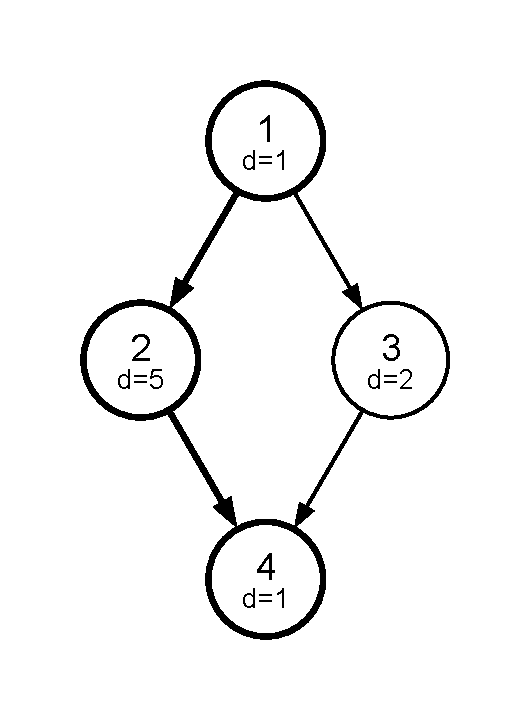
\includegraphics[width=0.3\linewidth]{fig01_example/fig01_example.pdf}
  \caption{The running example. Node durations $1, 5, 2, 1$; LongestPath is
  critical through nodes $1, 2, 4$ and ShortestPath through $1, 3, 4$.}
  \label{fig:cpm-example}
\end{figure}

Accumulation replaces the order by a sum, and the meeting in the middle
changes meaning. The total at a target $t$ expands to
$\sum_v m_{v} d_v + \sum_{(u,v)} m_{v} w_{uv}$, where $m_v$ counts the
directed routes from $v$ to the target, so a node influences the total not
through one best path but once per route, and the reverse traversal that
computes the counts, seeded with $m_t = 1$, is the adjoint of the forward
map. The count is the derivative of the total with respect to the node's
value, the product $m_v d_v$ is the node's share of the total, and under a
budget $B$ the room left to the node is $(B - F_t)/m_v$, headroom divided
across its routes. On the running example the total at node $4$ is $10$ and
node $1$ counts twice, once through each branch. Both kernels touch each
edge a constant number of times, so every mode costs $O(|V|+|E|)$ whatever
the operators are.

\section{Interval Analysis}
\label{sec:cpm-interval}

Uncertainty divides the toolkit's quantities along a single line, and the
line is monotonicity. Every forward quantity grows when any input grows, so
with interval inputs its exact bounds are two crisp runs of the scalar
kernel, one at the lower corner of the input box and one at the upper, and
interval arithmetic never enters. Margins sit on the other side of the
line. A margin is a difference of two monotone quantities that share their
inputs, it is not monotone in anything, and the hardness results of
Section~\ref{sec:cpm-grounding} live precisely there. Running the scalar
algorithms on an overloaded interval type would blur this line rather than
respect it, ranking overlapping intervals through a partial order that
cannot rank them and subtracting dependent quantities as though they were
independent. The toolkit instead computes each interval quantity by the
scheme its structure permits. Forward quantities are exact for the price of
two runs. Margins come either as a sound enclosure derived from those exact
bounds, declared conservative in the result it returns, or exactly, and an
exact value and an enclosure are never allowed to look alike.

\section{Exact Interval Floats: the Domination Split}
\label{sec:cpm-split}

Throughout this section the mode is LongestPath, durations $d_u$ lie in
intervals, delays are fixed, and $f_v = P - \mathrm{through}_v \ge 0$ is the
float of node $v$. An interval-valued delay reduces to this setting by
subdividing its edge with a node that carries the delay as its duration. The
question is the exact range of $f_v$ over the box of duration configurations.

\begin{proposition}[Corner sufficiency]
\label{prop:cpm-corner}
With all other durations fixed, $f_v$ is a monotone function of any single
duration $d_u$. Consequently the extremes of $f_v$ over the box are attained
at corner configurations.
\end{proposition}

\begin{proof}
A path visits a node at most once, so as a function of $x = d_u$ every path
length is either constant or affine with slope one. Hence
$P(x) = \max(C_0,\, C_1 + x)$, where $C_1$ is the best path through $u$ and
$C_0$ the best avoiding it, and likewise
$\mathrm{through}_v(x) = \max(A_0,\, A_1 + x)$ over the paths through $v$.
Each has one breakpoint with slope $0$ then $1$. If $P$'s breakpoint comes
first their difference has slope pattern $0, +1, 0$, otherwise $0, -1, 0$,
and in both cases $f_v$ is monotone in $x$ on the whole line. For the
corner claim, push any coordinate to whichever endpoint does not worsen the
objective, which monotonicity permits, and repeat per coordinate until the
configuration is a corner.
\end{proof}

\begin{lemma}[Incomparable coordinates]
\label{lem:cpm-incomparable}
If no complete path contains both $u$ and $v$, then $f_v$ is nondecreasing
in $d_u$, whatever the other durations are.
\end{lemma}

\begin{proof}
No through-$v$ path contains $u$, so $\mathrm{through}_v$ does not depend on
$d_u$, while $P$ is nondecreasing in it.
\end{proof}

\begin{lemma}[Dominated coordinates]
\label{lem:cpm-dominated}
If every complete path through $u$ also passes $v$, and in particular if
$u = v$, then $f_v$ is nonincreasing in $d_u$, whatever the other durations
are.
\end{lemma}

\begin{proof}
Suppose increasing $d_u$ increases $P$. The new maximiser must contain $u$,
hence $v$, hence it is a through-$v$ path, so $\mathrm{through}_v$ rises to
equal $P$ and the float drops to zero. If $P$ does not increase, the float
cannot rise because $\mathrm{through}_v$ is nondecreasing in every duration.
\end{proof}

The two lemmas cover every duration except those in the \emph{bypass set}
\[
H_v \;=\; \{\, u : \text{some complete path contains both } u \text{ and } v,
\text{ and some complete path contains } u \text{ but not } v \,\},
\]
the nodes that share a route with $v$ yet can also route around it.
Figure~\ref{fig:cpm-bypass} shows the three classes around one node.

\begin{figure}[htbp]
  \centering
  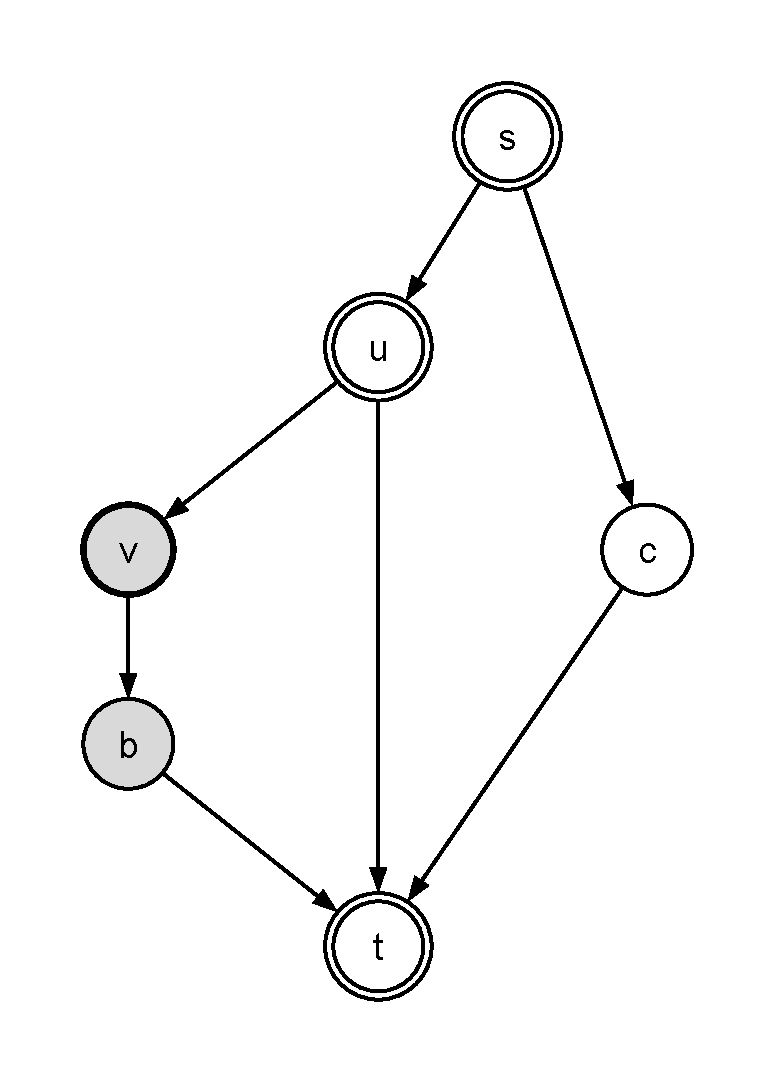
\includegraphics[width=0.5\linewidth]{fig02_bypass/fig02_bypass.pdf}
  \caption{Duration classes relative to node $v$. Shaded nodes are dominated
  by $v$ (every complete route through them passes $v$), the unfilled node is
  incomparable to it, and double-bordered nodes form the bypass set $H_v$:
  they share routes with $v$ and can also route around it.}
  \label{fig:cpm-bypass}
\end{figure}

\begin{theorem}[Exactness of the domination split]
\label{thm:cpm-split}
The maximum of $f_v$ over the box is attained at a corner with every
incomparable duration at its upper bound, every dominated duration at its
lower bound, and the bypass durations at some corner of $H_v$. The minimum is
attained dually. Enumerating the $2^{|H_v|}$ bypass corners with the
remaining durations pinned therefore yields the exact float range of $v$.
\end{theorem}

\begin{proof}
By Proposition~\ref{prop:cpm-corner} an optimum lies at a corner. The three
classes partition the durations. At an optimal corner, moving an incomparable
duration to its upper bound cannot decrease the maximum by
Lemma~\ref{lem:cpm-incomparable}, and moving a dominated duration to its
lower bound cannot decrease it by Lemma~\ref{lem:cpm-dominated}, so some
optimal corner has the pinned pattern and lies within the enumerated set.
\end{proof}

The cost is $2\sum_v 2^{|H_v|}$ crisp propagations, one maximising and one
minimising sweep per node, against $2^k$ for exhaustive enumeration of all
$k$ interval durations, and the exponent has
moved from the size of the problem to the reconvergent width around each
node. One exhaustive sweep serves every node simultaneously, so the
implementation runs whichever of the two is cheaper and is never worse than
exhaustive enumeration. Some instances must remain hard, because the general
problem is NP-hard \cite{chanas2002complexity}, and the split shows exactly
where the hardness sits: in networks whose bypass sets are large.

The bypass set is a reconvergence measure, and this is where the toolkit
touches the structural theme of Chapter~\ref{ch:diamond-module} without ever
calling its module. Both analyses pay for routes that divide and meet again,
the decomposition module per join through the nodes it must fix, the split
per node through $H_v$. The two sets index reconvergence at different
granularities, neither contains the other in general, and neither computation
uses the other.

\section{Case Studies}
\label{sec:cpm-cases}

Every number in this section is produced by the toolkit and certified
against an independent computation. The certification corpus contains nine
networks. On the seven where full path enumeration is affordable, forward
values, through-values, margins and critical sets of every mode agree with a
brute-force path oracle to within $3 \times 10^{-14}$, and on the remaining
two the results pass invariant and sampling checks. Interval results are certified
against exhaustive corner enumeration driven by the same path oracle, and
the domination split agrees with exhaustive enumeration everywhere both can
run.

\subsection{One network, four questions}
\label{sec:cpm-water}

The wastewater treatment network of 32 nodes and 66 edges shows how much
one set of inputs can say. Its stage processing times and pipeline delays
fix the minimum release timeline at 45 units, carried by the chain
$3 \to 11 \to 19 \to 27$ with a second chain $6 \to 14 \to 22 \to 30$ only
1.5 units behind (Table~\ref{tab:cpm-water-longest}). Stage 6 alone carries
slack 1 rather than 1.5, since its edge onto stage 11 lets it feed the
critical chain as well. Read for the opposite extreme, the
same inputs put the fastest achievable delivery at 15 units, and not along
one route. The twelve margin-zero stages and the eighteen tight
dependencies between them form a system of tied routes drawing on three
of the eight sources, sharing no stage with the critical chain, and the nearest
alternative stage sits 1.5 units behind the tie
(Figure~\ref{fig:cpm-chains}). The two extremal readings of one network
differ not only in which stages they select but in the shape of what they
select, a single thread against a redundant lattice.

\begin{figure}[htbp]
  \centering
  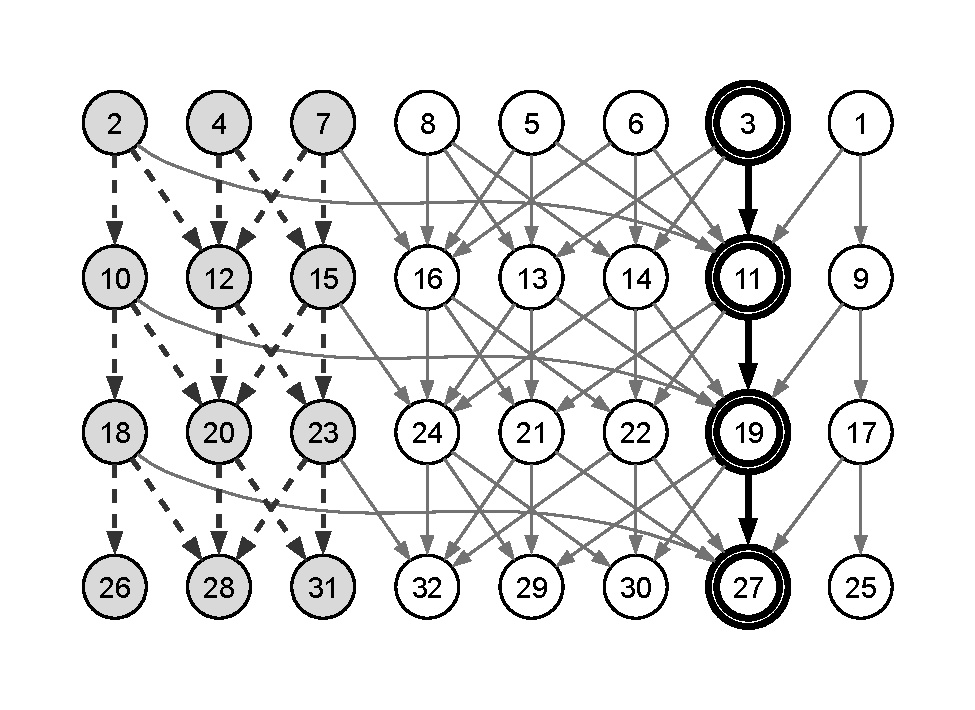
\includegraphics[width=0.92\linewidth]{fig04_chains/fig04_chains.pdf}
  \caption{The water network read for both extremes. The bold
  double-bordered chain sets the minimum release timeline of 45 units. The
  shaded stages and dashed edges form the tied-fastest route system, every
  path through which completes in 15 units. The two readings share no
  stage.}
  \label{fig:cpm-chains}
\end{figure}

\begin{table}[htbp]
\centering
\caption{LongestPath on the water network: completion 45 along the critical
chain, with the second chain behind it.}
\label{tab:cpm-water-longest}
\small
\renewcommand{\arraystretch}{1.15}
\begin{tabular}{lll}
\toprule
Node & Completion & Slack \\
\midrule
27 & 45.0 & 0 \\
19 & 33.0 & 0 \\
11 & 21.0 & 0 \\
3 & 9.0 & 0 \\
30 & 43.5 & 1.5 \\
22 & 31.5 & 1.5 \\
14 & 19.5 & 1.5 \\
6 & 8.0 & 1.0 \\
\bottomrule
\end{tabular}
\end{table}

Read as load rather than schedule, the same network delivers 480 units to
its busiest outlet, and the stages that drive that figure are not the ones
the completion times point at. The largest completions sit downstream where
load gathers, but the leverage sits upstream at stages 3, 6 and 5, each
reaching the outlet along seven distinct routes, so a unit added at any of
them arrives seven times. Under a budget ten percent above the current
total those three stages can each grow by less than seven units, while
stage 14, on two routes, has room for 24
(Table~\ref{tab:cpm-water-allowance}). Contribution and room order the
stages differently, which is the information a capacity decision needs and
which no scheduling slack could express.

\begin{table}[htbp]
\centering
\caption{Accumulation on the water network under a budget of 528 units at
outlet 27 (current total 480). Allowance is headroom divided by path
multiplicity.}
\label{tab:cpm-water-allowance}
\small
\renewcommand{\arraystretch}{1.15}
\begin{tabular}{llll}
\toprule
Node & Contribution & Multiplicity & Allowance \\
\midrule
3 & 63 & 7 & $+6.9$ \\
6 & 56 & 7 & $+6.9$ \\
5 & 35 & 7 & $+6.9$ \\
1 & 30 & 5 & $+9.6$ \\
11 & 27 & 3 & $+16$ \\
8 & 24 & 6 & $+8$ \\
14 & 16 & 2 & $+24$ \\
\bottomrule
\end{tabular}
\end{table}

Uncertainty then tests how much of the deterministic story survives. With
every one of the 32 stage durations widened to $\pm 20$ percent, exhaustive corner enumeration would
require $2^{32}$ propagations, roughly $4.3 \times 10^{9}$. The domination
split required $2{,}269{,}328$, a factor of $1{,}892$ fewer, with the largest
bypass set holding 18 of the 32 durations. The answer changes how the deterministic result must be
read. Under full uncertainty no stage is necessarily critical, and exactly
nine of the 32 are possibly critical. The single deterministic critical
chain dissolves into a nine-candidate set (Figure~\ref{fig:cpm-floats}),
and 23 stages are provably incapable of becoming critical anywhere in the
uncertainty box. A Monte
Carlo attack on the same bounds, fifty thousand sampled configurations,
produced no violation and reached every bound at every node.

\begin{figure}[htbp]
  \centering
  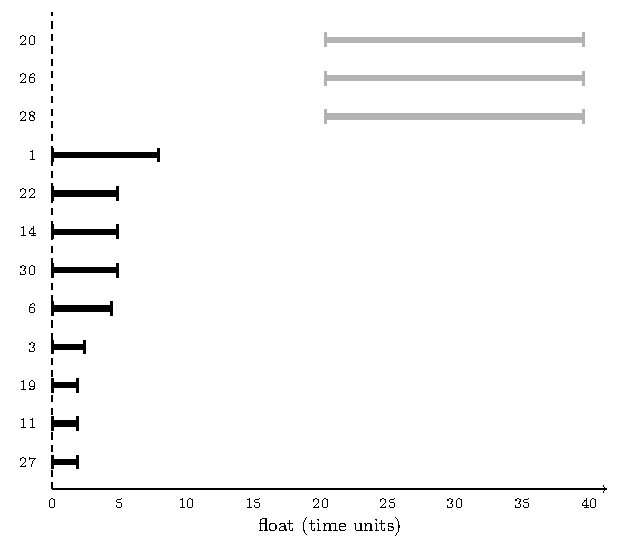
\includegraphics[width=0.82\linewidth]{fig06_floats/fig06_floats.pdf}
  \caption{Exact float bounds on the water network with every duration at
  plus or minus 20 percent. Black bars are the nine possibly-critical
  stages, whose lower bounds reach zero. Grey bars are three of the 23
  stages whose floats stay provably positive everywhere in the
  uncertainty box.}
  \label{fig:cpm-floats}
\end{figure}

\subsection{The most reliable route}
\label{sec:cpm-drone}

The drone medical delivery network of 782 nodes, 2,789 edges, 33 launch
sites and 323 destinations poses a multiplicative question, which route
delivers with the highest end-to-end success. The factors are the study's
own component success rates, node priors between 0.75 and 0.95 and
per-link probabilities between 0.70 and 0.95, so nothing in the scenario
is invented. The best route in the network compounds to a success factor
of 0.787, and it is a single direct leg from launch site 380 to
destination 393. That brevity is structural rather than accidental. The
strongest leg the data permits compounds its link and node factors to
0.9025, so every leg a route adds costs at least 9.8 percent of its
success, and no amount of component quality along a longer route can
repay that arithmetic. Route brevity is the currency of the
multiplicative reading, which nothing in an additive analysis of the same
network would reveal.

\begin{table}[htbp]
\centering
\caption{The five best-served destinations by single-route success. At
the other end of the scale, 104 of the 323 destinations fall below 0.5 on
even their best route.}
\label{tab:cpm-drone}
\small
\renewcommand{\arraystretch}{1.15}
\begin{tabular}{ll}
\toprule
Destination & Best-route success \\
\midrule
393 & 0.787 \\
325 & 0.771 \\
209 & 0.747 \\
248 & 0.742 \\
125 & 0.734 \\
\bottomrule
\end{tabular}
\end{table}

Read per destination rather than globally, the forward values become a
service-level map, and the map is unequal (Figure~\ref{fig:cpm-service}). The five best-served
destinations sit within seven percent of the optimum
(Table~\ref{tab:cpm-drone}), while the weakest destination in the network
can be reached with success 0.108 by its best route, and for 104 of the
323 destinations, roughly one in three, even the best single route
succeeds less than half the time. No routing decision alone can serve a
third of this network reliably, and where that matters the remedy is
structural, stronger components on the thin corridors or genuinely
redundant routes. Judging that redundancy is the neighbouring question,
because a destination poorly served by its best single route may still be
reliably reached when every route counts at once, which is the
reachability reading of Chapter~\ref{ch:probability-toolkit}. The two
readings separate route choice from system adequacy, and a delivery
planner for this network needs both. Two thousand randomly sampled routes
never exceeded the reported optimum and one reached it exactly, and the
optimum itself is the product of three published input values, checkable
by hand.

\begin{figure}[htbp]
  \centering
  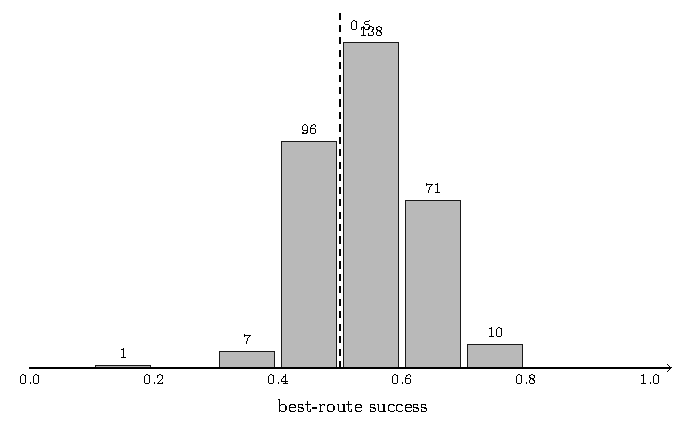
\includegraphics[width=0.78\linewidth]{fig05_service/fig05_service.pdf}
  \caption{Best-route success across the 323 drone destinations. Left of
  the dashed line at 0.5 lie the 104 destinations that no single route
  serves reliably.}
  \label{fig:cpm-service}
\end{figure}

\subsection{The boundary}
\label{sec:cpm-boundary}

Dense mesh reconvergence is where the split's advantage disappears. On a
five-by-five grid DAG with all 25 durations interval-valued, the bypass sets
hold up to 23 of the 25 durations and the split would need more propagations
than one shared exhaustive sweep, so the never-worse rule abandons the split
there and the instance stands at the exhaustive boundary itself. The hardness
results guarantee that some regime behaves this way, and it is the same
regime in which the sets of nodes the probability toolkit must fix and
enumerate explode. Mapping the boundary is part of the result rather than a
qualification of it. Timings are reported only as measured. The water
analyses run in 53 microseconds per pass for the additive modes and 7 for
accumulation, the drone network in 1.8 milliseconds, and the exhaustive
comparisons are quantified by run counts rather than by extrapolated
wall-time.

\section{Genericity}
\label{sec:cpm-genericity}

The boundary of the toolkit is drawn by the algebra rather than by the
implementation. A new quantity joins by exhibiting its operator pair, and
the pair earns its backward pass the way the shipped ones did, by carrying
a residual or by being linear. The obligations are laws, verified on
sampled values before a mode is accepted, so an extension can never
silently acquire a backward pass its algebra does not support. The kernels
are generic over the value they propagate, and interval support is a scheme
wrapped around crisp runs rather than a property of a value type, which is
what keeps its exactness claims provable.

The nearest extensions follow the existing arguments. The shortest-path
dual of the domination split mirrors Section~\ref{sec:cpm-split} and awaits
only the line-by-line derivation. Interval-valued delays reduce to interval
durations by subdividing their edges. Further out, neighbouring nodes have
overlapping bypass sets and therefore overlapping corner evaluations, an
economy of the kind the hash-consed store of Chapter~\ref{ch:diamond-module}
already practises for diamonds.

\section{Summary}
\label{sec:cpm-summary}

The toolkit reads one graph object in two directions. Forwards it computes
the extremal value of any quantity that accumulates along dependency paths.
Backwards it computes the room each component has before that value moves,
wherever the quantity's algebra defines such a reading, which is the
condition every shipped mode satisfies and every future mode must. The
classical critical path method is the default instance rather than the
design, and the sum family reports sensitivities and allowances because
that is what its mathematics defines. Under interval uncertainty the
forward quantities stay exact for the price of two crisp runs. The floats
are exact through the domination split, whose correctness rests on three
short proofs and whose cost grows with the reconvergent width around each
node rather than with the number of uncertain inputs. That width stayed
small enough on a real network to solve a 32-duration instance beyond the
reach of exhaustive enumeration, and it does not stay small on dense
meshes. Every number reported in this chapter is certified
against an independent oracle, an exhaustive enumeration or a sampling
attack.

\ifdefined\maindoc
% do nothing
\else
\printbibliography
\end{document}
\fi
